\documentclass[aspectratio=169,11pt]{beamer}
\usepackage[T1]{fontenc}
\usepackage[utf8]{inputenc}
\usepackage{lmodern}
\usepackage{amsmath,amssymb,booktabs,tabularx,array}
\usepackage[noend]{algpseudocode}
\usepackage{listings}
\usepackage{tikz,pgfplots}
\usetikzlibrary{arrows.meta,positioning,calc,fit,backgrounds}
\pgfplotsset{compat=1.18}
% The paper's paragraph helper shares a name with Beamer's example environment.
% No example environment is used in this deck.
\let\example\relax
% Shared vocabulary and editable diagram styles for paper and Beamer.
\definecolor{Ink}{HTML}{17324D}
\definecolor{Teal}{HTML}{087F8C}
\definecolor{Amber}{HTML}{A8670A}
\definecolor{Pale}{HTML}{EEF5F7}
\definecolor{Muted}{HTML}{526374}
\newcommand{\revision}{498dea0}
\newcommand{\snapshotdate}{25 November 2026}
\newcommand{\SAT}{\operatorname{SAT}}
\newcommand{\UNSAT}{\operatorname{UNSAT}}
\newcommand{\True}{\mathsf{true}}
\newcommand{\False}{\mathsf{false}}
\newcommand{\code}[1]{\texttt{\detokenize{#1}}}
\newcommand{\example}[1]{\paragraph{\textcolor{Teal}{#1}}}
% Source pointers remain in the editable text and evidence index.
\newcommand{\source}[1]{\par}
\tikzset{stage/.style={draw=Ink,thick,rounded corners=2pt,align=center,fill=Pale,minimum height=1.05cm,text width=2.65cm,font=\small},
  flow/.style={-{Stealth[length=2mm]},thick,draw=Teal},
  annotation/.style={font=\scriptsize,align=center,text=Muted}}

% Permanent links to the exact example texts preserved in the source snapshot.
\newcommand{\orderurl}{https://github.com/unibuc-cs/spelcheck/blob/498dea06df250964013b2abb2b06c94d341b223b/specs/order/requirements.md}
\newcommand{\authbaseurl}{https://github.com/unibuc-cs/spelcheck/blob/498dea06df250964013b2abb2b06c94d341b223b/specs/auth_change/openspec/specs/auth/spec.md}
\newcommand{\authchangeurl}{https://github.com/unibuc-cs/spelcheck/blob/498dea06df250964013b2abb2b06c94d341b223b/specs/auth_change/openspec/changes/admin-never-locked/specs/auth/spec.md}
\newcommand{\authfullurl}{https://github.com/unibuc-cs/spelcheck/blob/498dea06df250964013b2abb2b06c94d341b223b/specs/auth_openspec/spec.md}
\newcommand{\deletionurl}{https://github.com/unibuc-cs/spelcheck/blob/498dea06df250964013b2abb2b06c94d341b223b/specs/delete_property/requirements.md}

% A restrained, editable Beamer theme. Main-frame count excludes the appendix.
\usefonttheme{professionalfonts}
\setbeamertemplate{navigation symbols}{}
\setbeamertemplate{headline}{}
\pdfstringdefDisableCommands{\def\translate#1{#1}}
\setbeamertemplate{itemize item}{\color{Teal}\small\textbullet}
\setbeamertemplate{itemize subitem}{\color{Teal}\small\textendash}
\setbeamercolor{normal text}{fg=Ink,bg=white}
\setbeamercolor{structure}{fg=Teal}
\setbeamercolor{frametitle}{fg=Ink,bg=white}
\setbeamercolor{title}{fg=Ink}
\setbeamercolor{alerted text}{fg=Amber}
\setbeamerfont{normal text}{size=\fontsize{12.5}{16}\selectfont}
\setbeamerfont{frametitle}{size=\fontsize{23}{27}\selectfont,series=\bfseries}
\setbeamerfont{title}{size=\fontsize{29}{34}\selectfont,series=\bfseries}
\setbeamerfont{subtitle}{size=\fontsize{17}{22}\selectfont}
\setbeamersize{text margin left=10mm,text margin right=10mm}
\newif\ifmainframe
\mainframetrue
\setbeamertemplate{frametitle}{%
  \vspace{1mm}%
  {\fontsize{8.5}{10}\selectfont\color{Muted}%
    \ifmainframe\insertsectionnumber\quad\insertsectionhead
    \else Technical appendix\fi\par}%
  \vspace{0.5mm}%
  {\usebeamerfont{frametitle}\insertframetitle\par}%
  \vspace{1mm}}
\setbeamertemplate{footline}{%
  \begin{beamercolorbox}[wd=\paperwidth,ht=3mm,dp=2.4mm,rightskip=10mm]{normal text}
    \hfill{\fontsize{7.5}{9}\selectfont\color{Muted}\insertpagenumber}
  \end{beamercolorbox}}
\setlength{\parskip}{3pt}
\setlength{\emergencystretch}{2em}
\renewcommand{\arraystretch}{1.2}
% Keep source pointers in the .tex file without printing them on slides.
\newcommand{\slidesource}[1]{\vfill}
\newcommand{\lead}[1]{{\large\color{Teal}#1\par}\vspace{1mm}}
\newcommand{\takeaway}[1]{\par\vspace{0.5mm}{\color{Teal}#1\par}}
% In-body navigation stays separate from the page-number-only footer.
\newcommand{\details}[2]{{\fontsize{8.5}{10}\selectfont\color{Muted}\hyperlink{#1}{Details: Appendix #2}}}
\newcommand{\backto}[2]{{\fontsize{8.5}{10}\selectfont\color{Muted}\hyperlink{#1}{Back to #2}}}
\newcommand{\backuptext}{\fontsize{10.8}{13.2}\selectfont\setlength{\parskip}{3pt}}
\newcommand{\talknote}[2]{\note{\textbf{Time: #1.}\par #2}}
\lstset{basicstyle=\ttfamily\fontsize{9.5}{11.5}\selectfont,
  columns=fullflexible,keepspaces=true,showstringspaces=false,
  breaklines=true,frame=single,rulecolor=\color{Teal!35},
  backgroundcolor=\color{Pale},aboveskip=5pt,belowskip=5pt,
  xleftmargin=3pt,xrightmargin=3pt,framexleftmargin=3pt,framexrightmargin=3pt}
\tikzset{slidearrow/.style={-{Stealth[length=2.2mm]},thick,Teal},
  slidetext/.style={align=left,text=Ink,font=\normalsize}}

\ifdefined\speakersnotes
  \setbeameroption{show only notes}
\else
  \setbeameroption{hide notes}
\fi
\hypersetup{pdftitle={speccheck: requirements analysis with LLMs and Z3},pdfsubject={31-slide academic briefing with 11 appendix slides, revision 498dea0}}
\title{speccheck: requirements analysis with LLMs and Z3}
\begin{document}
\usebeamerfont{normal text}

% MAIN 01 / 31

\begin{frame}[plain,label=main01]
\vspace{5mm}
{\color{Teal}\large REQUIREMENTS ANALYSIS\par}
\vspace{4mm}
{\usebeamerfont{title}speccheck\par}
\vspace{2mm}
{\usebeamerfont{subtitle}From requirements to questions for review\par}
\vspace{8mm}
{\large LLMs translate. Z3 checks the formulas.\\We keep the interpretation choices visible.\par}
\vfill
{\color{Muted}\normalsize Design, evidence and next steps\par}
{\small\snapshotdate\quad /\quad revision \code{498dea0}\par}
\talknote{0:30}{This is speccheck at revision 498dea0. The talk moves from a requirements problem to the approach, four evaluation questions, limitations and next work. This is an independent research prototype, not a reconstruction or assessment of Kiro's implementation. The main talk is about thirty-four minutes.}
\end{frame}

\section{Problem and example}

\subsection{The project before the change}

% MAIN 02 / 31

\begin{frame}[fragile,label=main02]{The project before the change}
\lead{Authentication already has a specification with four scenarios.}
{\small \href{\authbaseurl}{\textcolor{Teal}{\code{openspec/specs/auth/spec.md}}}\quad Existing capability: \code{auth}.\par}
\begin{columns}[T,onlytextwidth]
\column{.46\textwidth}
\textbf{Login}\par
R1: valid credentials, grant access.\\
R2: invalid credentials, deny access.\par
\vspace{2mm}
\textbf{Account Lockout}\par
R3: failed attempts reach five, lock.\\
R4: password for a locked account, deny access.
\column{.50\textwidth}
{\small Literal base excerpt; selected lines.\par}
\begin{lstlisting}
### Requirement: Account Lockout
#### Scenario: Lockout threshold
- **WHEN** the number of failed attempts on an account reaches 5
- **THEN** the system locks the account
\end{lstlisting}
\end{columns}
\takeaway{The delta will refer to this project's requirement and scenario names.}
\slidesource{specs/auth_change/openspec/specs/auth/spec.md; specs/auth_change/merged.md}
\talknote{1:00}{Start with the project before the proposed change. This is a repository-authored teaching example, not an independently validated production system. The left column summarizes its four scenarios and uses labels from the saved merged example. The right excerpt copies the requirement and scenario headers and the scenario body, omitting the requirement's SHALL sentence and blank lines. The full source is linked. The baseline has existing findings, including an R1/R4 conflict; we do not claim it is logically clean. What matters next is whether the delta introduces a new interaction.}
\end{frame}

\subsection{The question and the route}

% MAIN 03 / 31

\begin{frame}[label=main03]{The question and the route}
\lead{Can LLM translations and solver checks give us useful questions for review?}
\begin{tabularx}{\textwidth}{@{}lX@{}}
\toprule
Part & What we will establish \\
\midrule
1. Problem and example & Authentication rules and our review questions. \\
2. Findings & Four questions, their formulas and concrete cases. \\
3. Method & How words become formulas we can inspect. \\
4. Changes & OpenSpec baseline, delta and findings. \\
5. Evaluation & What the experiments found, including extra alarms. \\
6. Limits and next steps & Where the approach needs more work. \\
\bottomrule
\end{tabularx}
\talknote{0:45}{Authentication is the running example for all four check definitions and for OpenSpec changes. Deletion is one brief supporting illustration of assumptions. The paper retains order processing as a separate worked example. The studies measure detection and variation. Whether this saves reviewers time or improves their decisions still needs independent study. Detailed algorithms are in the appendix.}
\end{frame}

\subsection{Four questions for the same project}

% MAIN 04 / 31

\begin{frame}[label=main04]{Four questions for the same project}
\begin{tabularx}{\textwidth}{@{}lX@{}}
\toprule
Finding & Authentication example \\
\midrule
\textbf{Conflict} & Five failures: lock an administrator or forbid lockout? \\
\textbf{Gap} & Without R2, what handles an incorrect password? \\
\textbf{Ambiguity} & Does ``reaches five'' mean exactly five, or five and above? \\
\textbf{Generated scenario} & May access be granted without a password submission? \\
\bottomrule
\end{tabularx}
\takeaway{We will show the rule, the logical question and a concrete situation for each.}
\talknote{0:45}{These four questions organize the whole method. The baseline is the same authentication project throughout. For conflict we add the actual administrator exception. For the gap we separately remove the invalid-password response. For ambiguity and allowed behavior we return to the four baseline scenarios. These are not four defects asserted in one unchanged document. Generated consequences can be allowed or ruled out and are not automatically defects.}
\end{frame}

\section{Findings}

\subsection{The predicates we will use}

% MAIN 05 / 31

\begin{frame}[label=main05]{The predicates we will use}
\setlength{\parskip}{2pt}
\begin{columns}[T,onlytextwidth]
\column{.46\textwidth}
\begingroup\small
\begin{tabular}{@{}ll@{}}
\toprule
$p$ & password submitted \\
$v$ & password correct \\
$g,d$ & access granted, access denied \\
$n$ & failed-attempt count \\
$\ell$ & account locked \\
$h$ & administrator account \\
\bottomrule
\end{tabular}\par
\endgroup
\column{.50\textwidth}
\textbf{Baseline examples}\par
R1: $(p\land v)\Rightarrow g$\par
R3: $(n=5)\Rightarrow\ell$\par
{\small R3 has another reading: $n\ge5$.\par}
\vspace{2mm}
\textbf{Proposed addition}\par
R5: $h\Rightarrow\neg\ell$
\end{columns}
\vspace{2mm}
Rule form: $\phi_i=\underbrace{a_i}_{\text{condition}}\Rightarrow\underbrace{c_i}_{\text{outcome}}$,\quad $\Phi=\bigwedge_i\phi_i$.\par
{\small SAT: a case exists. UNSAT: none exists. Unknown proves neither.\par}
\takeaway{Each case is one snapshot, with no sequence of events.}\par\details{app-a}{A}
\talknote{1:00}{These are short editorial names for the saved authentication symbols. Plain v means password_correct, not stock as in the paper's separate order example. Subscript a_i and c_i mean a rule's antecedent and consequence. In formulas Phi denotes their conjunction. Grant and deny are separate saved symbols; we have not silently made them logical negations. R3's selected saved antecedent is n=5 with no password-submitted guard, despite trigger metadata. The proposed administrator rule is not in the baseline. A witness establishes a property of this encoding, not a history of the running system.}
\end{frame}

\subsection{Conflict: obligations cannot coexist}

% MAIN 06 / 31

\begin{frame}[label=main06]{Conflict: obligations cannot coexist}
\lead{Baseline + administrator exception: five failed attempts.}
{\small Trigger $T=h\land(n=5)$. R3 requires $\ell$; added R5 requires $\neg\ell$.\par}
\begin{center}
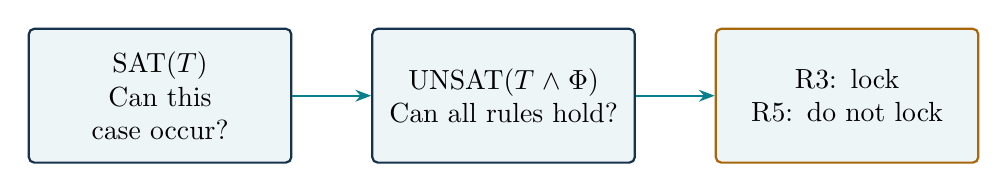
\begin{tikzpicture}[node distance=10mm,stage/.append style={text width=3.1cm,font=\normalsize,minimum height=17mm}]
\node[stage] (a) {$\SAT(T)$\\Can this case occur?};
\node[stage,right=of a] (b) {$\UNSAT(T\land\Phi)$\\Can all rules hold?};
\node[stage,right=of b,draw=Amber] (c) {R3: lock\\R5: do not lock};
\draw[flow] (a)--(b);\draw[flow] (b)--(c);
\end{tikzpicture}
\end{center}
\textbf{Witness:} an administrator account with five failed attempts.\par
\takeaway{Several rules clash. A case forbidden by one rule alone is handled as a ruled-out scenario.}\par\details{app-g}{G}
\talknote{1:15}{This is the same R3/R5 conflict as the saved OpenSpec change result. Five attempts works under both the exactly-five and at-least-five readings. T is feasible before imposing obligations, and adding all active rules is unsatisfiable. Neither R3 nor R5 by itself makes T impossible: one requires locked, the other requires not locked. This separates competing obligations from a single prohibition. The formal formula here omits assumptions for clarity; the implementation also performs an assumptions pass, bounds connected trigger groups at three, and reduces the unsatisfiable core. Unknown is not proof of a conflict.}
\end{frame}

\subsection{Gap: no conditional response applies}

% MAIN 07 / 31

\begin{frame}[label=main07]{Gap: no conditional response applies}
\lead{Separate variation: baseline without R2, the invalid-password response.}
\begin{center}
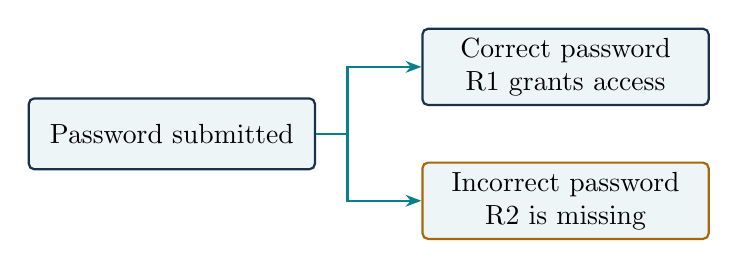
\begin{tikzpicture}[stage/.append style={font=\normalsize,text width=3.4cm,minimum height=9mm}]
\node[stage] (p) at (0,0) {Password submitted};
\node[stage] (yes) at (5,0.85) {Correct password\\R1 grants access};
\node[stage,draw=Amber] (no) at (5,-0.85) {Incorrect password\\R2 is missing};
\draw[flow] (p.east)--++(4mm,0)|-(yes.west);
\draw[flow] (p.east)--++(4mm,0)|-(no.west);
\end{tikzpicture}
\end{center}
\vspace{-1mm}
\textbf{Question:}\quad $\SAT\bigl(p\land\neg a_1\land\neg a_3\land\neg a_4\bigr)$?\par
\textbf{Witness:}\quad $p=\True,\ v=\False,\ \ell=\False,\ n=0$.\par
{\small R1, R3 and R4 are inactive. R5 is not part of this variation.\par}
\details{app-h}{H}
\talknote{1:15}{Use only the four baseline scenarios, then remove R2. A password is submitted and is incorrect, the account is unlocked, and failed_attempts_count is zero. The selected R3 antecedent n=5 is false; R1 and R4 are also false. The surviving rule set still reacts to password submission, so this is a handled-event coverage gap. This is an offline-checked construction, not a new saved model-server run or a claim that this delta exists in the repository. The original R1/R2 pair covers both password cases. The general event query fixes other event symbols false; p is the only event here. Quiet gaps may be intended, and this check is narrower than full business completeness.}
\end{frame}

\subsection{Ambiguity: interpretations differ}

% MAIN 08 / 31

\begin{frame}[label=main08]{Ambiguity: interpretations differ}
\lead{Original baseline: R3 says failed attempts ``reach 5''.}
\begin{columns}[T,onlytextwidth]
\column{.47\textwidth}
\textbf{A: exactly five}\par
$\phi_A=(n=5)\Rightarrow\ell$\par
\vspace{3mm}
\textbf{B: five or more}\par
$\phi_B=(n\ge5)\Rightarrow\ell$
\column{.49\textwidth}
\textbf{Distinguishing case}\par
$\SAT(\phi_A\oplus\phi_B)$\par
$n=6,\quad \ell=\False$\par
A allows this unlocked account.\\B rules it out.
\end{columns}
\vspace{2mm}
Samples and interpretation probes determine the review flag.\par
\takeaway{Z3 proves the formulas differ. It does not decide which English reading is intended.}\par\details{app-d}{D}\qquad\details{app-f}{F}
\talknote{1:30}{Return to the unchanged baseline rather than combining this with the gap variation. The saved model selected exactly five and retained at least five as an alternative. The saved probe uses six attempts and unlocked, matching this witness. XOR asks for a snapshot allowed by exactly one formula. A formal difference is not enough to establish ambiguity in natural language: sampling groups, entropy thresholds, interpretation probes and an optional second reader determine the review flag. Unusable or rejected formalizations can also appear as interpretation warnings. Unknown does not establish equivalence. We show how translations are obtained after this block.}
\end{frame}

\subsection{Generated scenarios: is this intended?}

% MAIN 09 / 31

\begin{frame}[label=main09]{Generated scenarios: is this intended?}
\begin{columns}[T,onlytextwidth]
\column{.48\textwidth}
\textbf{Allowed: original baseline}\par
R1: $(p\land v)\Rightarrow g$\par
$\SAT\bigl(\Phi_{\rm base}\land\neg(p\land v)\land g\bigr)$\par
\vspace{2mm}
$p=\False,\ g=\True$,\\$n=0,\ \ell=\False$.\par
Access is granted without a password submission. All four rules hold.
\column{.48\textwidth}
\textbf{Ruled out: with the exception}\par
R5: $h\Rightarrow\neg\ell$\par
$T=h\land p\land\ell$\par
$\SAT(T)$, but $\UNSAT(T\land\neg\ell)$.\par
\vspace{2mm}
An administrator is locked and submits a password. R5 alone rules this out.
\end{columns}
\takeaway{These are consequences to confirm, not automatically defects.}\par
{\small Generated scenarios are output examples. OpenSpec scenarios are the input text.\par}
\talknote{1:30}{The left snapshot is an offline-checked construction on the four baseline rules projected from the saved authentication formalization. Other Booleans are false; it also satisfies the saved domain facts, though the scenario search itself uses only rules. It says access is allowed without a submission event in this snapshot, not that no password was ever submitted in a past history. For the right panel, add the administrator exception. R4 and R5 have feasible simultaneous antecedents p and locked and admin; R5's consequence not locked alone makes that case impossible. The checker treats this as a ruled-out consequence rather than two competing obligations. An LLM subsequently judges which generated consequences are surprising enough to show.}
\end{frame}

\section{Method}

\subsection{From text to a review report}

% MAIN 10 / 31

\begin{frame}[label=main10]{From text to a review report}
\begin{center}
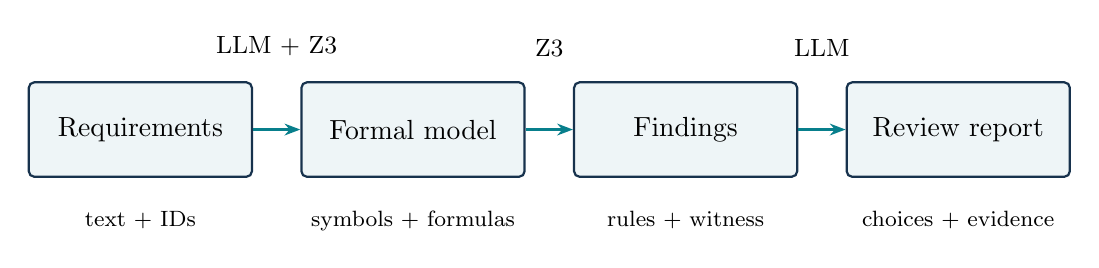
\begin{tikzpicture}[node distance=6mm,stage/.append style={font=\normalsize,text width=2.6cm,minimum height=12mm}]
\node[stage] (w) {Requirements};
\node[stage,right=of w] (m) {Formal model};
\node[stage,right=of m] (f) {Findings};
\node[stage,right=of f] (r) {Review report};
\draw[flow] (w)--node[above=8mm,font=\small]{LLM + Z3}(m);
\draw[flow] (m)--node[above=8mm,font=\small]{Z3}(f);
\draw[flow] (f)--node[above=8mm,font=\small]{LLM}(r);
\node[below=3mm,font=\footnotesize] at (w.south) {text + IDs};
\node[below=3mm,font=\footnotesize] at (m.south) {symbols + formulas};
\node[below=3mm,font=\footnotesize] at (f.south) {rules + witness};
\node[below=3mm,font=\footnotesize] at (r.south) {choices + evidence};
\end{tikzpicture}
\end{center}
\vspace{2mm}
\textbf{R3 through the pipeline}\quad Lockout text $\to$ explicit obligation
$\to$ conflict with R5 $\to$ a review question.
\takeaway{Saved formulas let us replay the solver without a model server.}\par\vspace{0.25mm}\details{app-k}{K}
\slidesource{speccheck/cli.py; speccheck/logic.py; speccheck/explain.py}
\talknote{1:00}{Follow the three transformations from requirements to a formal model, then findings, then a review report. Formalization combines LLM proposals with solver comparisons. Checks make no LLM calls. The reporting model words findings and judges which scenarios are worth showing. Python selects queries, groups translations and applies votes and filters. Saved formulas can be replayed without the reporting branch.}
\end{frame}

\subsection{Building the formal model}

% MAIN 11 / 31

\begin{frame}[label=main11]{Building the formal model}
\begin{center}
% Slide-scale overview: shorter labels preserve readable type.
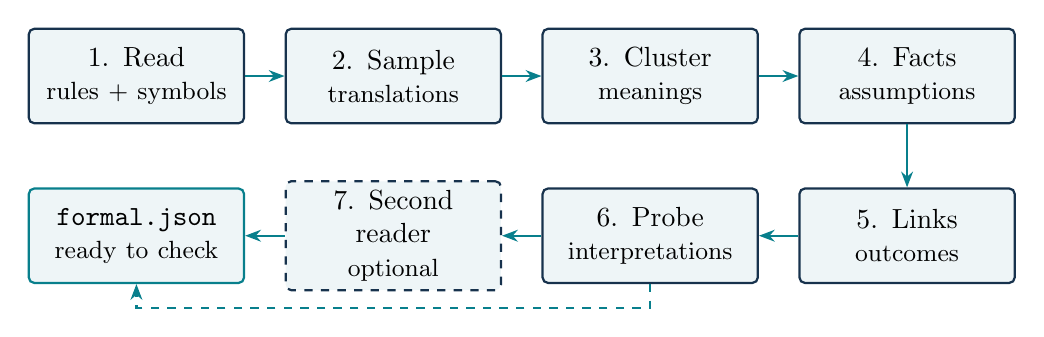
\begin{tikzpicture}[node distance=5mm,stage/.append style={font=\normalsize,text width=2.5cm,minimum height=12mm}]
\node[stage] (r) {1. Read\\\small rules + symbols};
\node[stage,right=of r] (s) {2. Sample\\\small translations};
\node[stage,right=of s] (c) {3. Cluster\\\small meanings};
\node[stage,right=of c] (f) {4. Facts\\\small assumptions};
\node[stage,below=8mm of f] (l) {5. Links\\\small outcomes};
\node[stage,left=of l] (p) {6. Probe\\\small interpretations};
\node[stage,left=of p,dashed] (x) {7. Second reader\\\small optional};
\node[stage,left=of x,draw=Teal] (o) {\texttt{formal.json}\\\small ready to check};
\draw[flow] (r)--(s);\draw[flow] (s)--(c);\draw[flow] (c)--(f);
\draw[flow] (f)--(l);\draw[flow] (l)--(p);\draw[flow] (p)--(x);\draw[flow] (x)--(o);
\draw[flow,dashed] (p.south) -- ++(0,-.3) -| (o.south);
\end{tikzpicture}

\end{center}
\vspace{1mm}
Authentication R3 passes from its words to a selected formula.
\takeaway{The default is eight samples and one vocabulary; the second reader is optional.}\par\vspace{0.25mm}\details{app-b}{B}
\slidesource{speccheck/formalize.py; speccheck/probe.py}
\talknote{0:45}{This map is the overview; the talk groups the steps by their purpose rather than following every loop. Sampling and grouping compare translations. Facts and links relate terms. Probes challenge interpretations and assumptions. An optional second model checks the selected reading using the same vocabulary. Full procedures are in the appendices. The default remains eight samples and one vocabulary. Optional incremental mode retains the old vocabulary and readings, selectively formalizes the new scenarios, and reruns the ordinary solver checks on the combined model. It excludes the second reader.}
\end{frame}

\subsection{Comparing translations}

% MAIN 12 / 31

\begin{frame}[fragile,label=main12]{Comparing translations}
\lead{Eight translations share one vocabulary. Z3 compares their meanings.}
\begin{columns}[T,onlytextwidth]
\column{.49\textwidth}
{\small Illustrative R1 translation, short names.\par}
\begin{lstlisting}
{
  "reading": "A correct password submission requires access.",
  "antecedent": "(and p v)",
  "consequent": "g"
}
\end{lstlisting}
\column{.47\textwidth}
\textbf{Same meaning?}\par
$\UNSAT(\phi_A\oplus\phi_B)$ means no case satisfies exactly one formula.\par
\vspace{2mm}

\begin{tikzpicture}[x=.48cm,y=.6cm]
\foreach \x in {0,...,4} {\fill[Teal] (\x,0) circle(.18);}
\foreach \x in {5,...,7} {\fill[Amber] (\x,0) circle(.18);}
\node[below,align=left,font=\small] at (3.5,-.35) {Illustrative split: 5 + 3\\two meanings, flagged ambiguous};
\end{tikzpicture}
\end{columns}
{\small Sampling temperature 0.7. Group sizes measure stability of the usable translations.\par}
\takeaway{Eight matching answers can still repeat the same mistake.}
\par\vspace{0.25mm}\details{app-b}{B}
\slidesource{speccheck/formalize.py: _translate, _judge, _group_by_meaning}
\talknote{1:30}{The JSON is illustrative and uses short names; saved models use descriptive names. Z3 compares whole implications using XOR and only merges them when it proves equivalence. The dots are constructed samples, not an experimental result. Five and three produce entropy about 0.662; accepted is H at most 0.4, ambiguous through 1, otherwise rejected. Rejected rules are omitted from the main checks. Low entropy is not a probability that the English meaning is correct. Unknown is not equivalence.}
\end{frame}

\subsection{Relating separate outcomes}

% MAIN 13 / 31

\begin{frame}[label=main13]{Relating separate outcomes}
\lead{Supporting example: deletion and audit retention.}
{\small D2 removes the record; D4 retains it. \href{\deletionurl}{\textcolor{Teal}{Read the requirements}}.\par}
{\small $d$: confirmation; $m$: removed; $k$: retained.\par}
\begin{center}
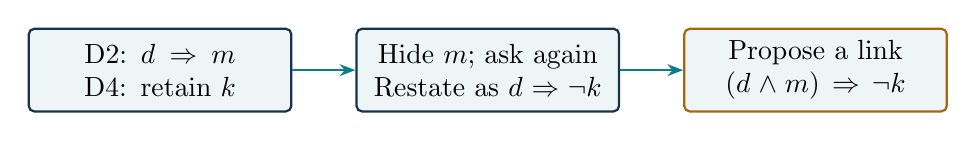
\begin{tikzpicture}[node distance=8mm,stage/.append style={text width=3.1cm,font=\normalsize}]
\node[stage] (a) {D2: $d\Rightarrow m$\\D4: retain $k$};
\node[stage,right=of a] (b) {Hide $m$; ask again\\Restate as $d\Rightarrow\neg k$};
\node[stage,right=of b,draw=Amber] (c) {Propose a link\\$(d\land m)\Rightarrow\neg k$};
\draw[flow] (a)--(b);\draw[flow] (b)--(c);
\end{tikzpicture}
\end{center}
Without the link, $m$ and $k$ can both hold. With it, confirmation exposes the clash.
\par{\small Abbreviated example: does ``remove'' mean erase, or hide while retaining an audit copy?\par}
\takeaway{Whether removal and retention conflict depends on what the words mean.}\par\vspace{0.25mm}\details{app-c}{C}\qquad\details{app-e}{E}
\slidesource{speccheck/formalize.py: _symbols_to_hide, _links}
\talknote{1:30}{The deletion formulas are abbreviated illustrations. A private outcome is used by no other rule. The system hides that symbol, asks for equivalent restatements using other outcomes, and retains a majority-supported link unless retained assumptions contradict it. Domain facts come from symbol descriptions. Outcome-pair questions ask whether two definite outcomes can coexist. The E18 evaluation isolates this last mechanism. Every added relation is defeasible: removal could mean hiding a record while retaining an audit copy.}
\end{frame}

\subsection{From evidence to a review question}

% MAIN 14 / 31

\begin{frame}[fragile,label=main14]{From evidence to a review question}
\vspace{0pt}
\begin{columns}[T,onlytextwidth]
\column{.49\textwidth}
{\small Saved authentication finding: selected fields.\par}
\begin{lstlisting}
{
  "type": "conflict",
  "rules": ["R3", "R5"],
  "when": {
    "failed_attempts_count": 5,
    "is_administrator": true
  },
  "about_change": true
}
\end{lstlisting}
\column{.47\textwidth}
\textbf{Illustrative review question}\par
An administrator reaches five failed attempts. R3 requires lockout; R5 forbids it. Which policy should change?\par
\vspace{2mm}
\textbf{Decision:} revise the lockout rule or the administrator exception.
\end{columns}
\takeaway{The rule IDs and concrete case make the question checkable.}\par\details{app-g}{G}
\talknote{0:45}{These selected JSON fields are copied from the saved authentication finding. The right-hand wording is a concise editorial question, not a saved LLM response. This conflict needs no background fact. Other findings can depend on assumed relations or carry doubt markers. Generated explanations need checking against the evidence; the author decides the policy. We next explain the OpenSpec delta structure that makes about_change meaningful.}
\end{frame}

\section{Changes}

\subsection{How a delta is organized}

% MAIN 15 / 31

\begin{frame}[fragile,label=main15]{How a delta is organized}
\vspace{0pt}
\setlength{\parskip}{2pt}
{\small The proposed change has its own folder. Its \code{auth} file targets the existing \code{auth} capability.\par}
\begin{lstlisting}
openspec/changes/admin-never-locked/
  specs/auth/spec.md
\end{lstlisting}
{\small Up to four sections. The merger applies them in this order:\par}
\begingroup\small
\begin{tabularx}{\textwidth}{@{}lX@{}}
\toprule
Section header & What it supplies \\
\midrule
\texttt{\#\# RENAMED Requirements} & \code{FROM:} old name; \code{TO:} new name. \\
\texttt{\#\# REMOVED Requirements} & Requirement name, followed by a reason. \\
\texttt{\#\# MODIFIED Requirements} & The full replacement text of one requirement. \\
\texttt{\#\# ADDED Requirements} & The full text of a new requirement. \\
\bottomrule
\end{tabularx}\par
\endgroup
{\small Requirements match by name. Later operations use the new name after a rename.\par}
\takeaway{An absent capability gets a specification from its ADDED requirements.}
\slidesource{speccheck/change.py: merge, _sections}
\talknote{1:00}{The base file is under openspec/specs/auth; this delta is under openspec/changes/admin-never-locked/specs/auth. The capability path connects them. The file needs only the sections relevant to its change; the administrator example uses ADDED alone. RENAMED uses FROM and TO lines whose values are Requirement headers. REMOVED's body explains why; it is not replacement policy. MODIFIED supplies the complete new body of the named requirement, not just edited lines. Requirements omitted from the delta stay unchanged. A new capability uses a previously absent path and ADDED content. The checker builds an analysis document and does not archive or overwrite baseline files.}
\end{frame}

\subsection{Which scenarios changed}

% MAIN 16 / 31

\begin{frame}[label=main16]{Which scenarios changed}
\lead{Inside a MODIFIED requirement, match scenarios by name.}
\begin{tabularx}{\textwidth}{@{}lX@{}}
\toprule
Status & How the merger assigns it \\
\midrule
\code{existing} & Same name and normalized text. \\
\code{modified} & Same name, different normalized text. \\
\code{added} & A new scenario name. \\
\code{removed} & Its requirement is removed, or the replacement omits its name. \\
\bottomrule
\end{tabularx}
{\small Example: copying \emph{Lockout threshold} keeps it existing; changing five to seven makes it modified. Omitting it from the full replacement removes it.\par}
\takeaway{Administrator delta: four existing scenarios and one added scenario.}
\slidesource{speccheck/change.py: _rewritten, _plain; specs/auth_change/}
\talknote{1:15}{The threshold edits are separate illustrations, not edits in the saved administrator delta. The actual change adds Administrator Access, with Administrators are never locked out; all four original scenarios remain existing. Matching uses exact scenario names and normalized bodies, not semantic equivalence. Normalization ignores case, whitespace and selected Markdown markers. A scenario rename has no dedicated operation: it can become removal plus addition. A MODIFIED block must include scenarios that are meant to remain. Full formalization labels the resulting document in order; these labels need not remain stable across arbitrary edits. The optional reuse mode preserves old base labels and tracks replaced readings separately.}
\end{frame}

\subsection{An OpenSpec change in context}

% MAIN 17 / 31

\begin{frame}[label=main17]{An OpenSpec change in context}
\lead{Authentication: add an administrator exception.}
{\small Project OpenSpec example: \href{\authbaseurl}{\textcolor{Teal}{base specification}} $\to$ \href{\authchangeurl}{\textcolor{Teal}{proposed change}}.\par}
\begin{center}
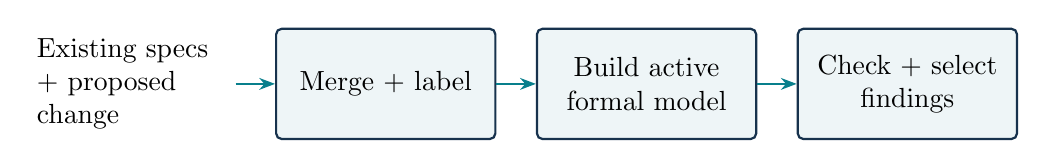
\begin{tikzpicture}[node distance=5mm,stage/.append style={font=\normalsize,text width=2.55cm,minimum height=14mm}]
\node[align=left,font=\normalsize,text width=2.4cm] (s) {Existing specs\\+ proposed change};
\node[stage,right=of s] (m) {Merge + label};
\node[stage,right=of m] (c) {Build active\\formal model};
\node[stage,right=of c] (f) {Check + select\\findings};
\draw[flow] (s)--(m);\draw[flow] (m)--(c);\draw[flow] (c)--(f);
\end{tikzpicture}
\end{center}
\vspace{2mm}
Existing R3: lock the account when failed attempts reach five.\\
Added R5: do not lock an administrator's account.
\takeaway{Check the combined rules, then select findings related to the change.}\par\vspace{0.25mm}\details{app-i}{I}
\slidesource{speccheck/change.py; specs/auth_change/}
\talknote{1:00}{This is the actual authentication OpenSpec base and proposed change. The links open the version used here. Merge applies rename, remove, modify and add operations, labels scenarios and records provenance. Scenario names and normalized text distinguish unchanged, changed, added and removed scenarios. Normalization is textual, not semantic equivalence. Deleted and replaced obligations are removed before analysis; tagged links and outcome-pair assumptions concerning them are pruned. Baseline files are not mutated. Findings are selected by changed rules, changed events or explicit removal attribution. Unchanged scenarios keep their provenance even inside a modified requirement. This is not a complete semantic before/after comparison.}
\end{frame}

\subsection{The administrator conflict}

% MAIN 18 / 31

\begin{frame}[fragile,label=main18]{The administrator conflict}
\vspace{0pt}
\begin{columns}[T,onlytextwidth]
\column{.59\textwidth}
{\small OpenSpec change: literal text, blank lines omitted.\par}
\begin{lstlisting}[basicstyle=\ttfamily\fontsize{9}{10.8}\selectfont]
## ADDED Requirements
### Requirement: Administrator Access
Administrators MUST always be able to reach the system.
#### Scenario: Administrators are never locked out
- **WHEN** the account belongs to an administrator
- **THEN** the system does not lock the account
\end{lstlisting}
\column{.37\textwidth}
{\small Authentication: saved fields.\par}
\begin{lstlisting}[basicstyle=\ttfamily\fontsize{9}{10.8}\selectfont]
"rules": ["R3", "R5"],
"when": {
  "failed_attempts_count": 5,
  "is_administrator": true
},
"about_change": true
\end{lstlisting}
At five, both readings require lockout. The exception forbids it.
\end{columns}
\takeaway{The R3/R5 conflict is selected; the older R1/R4 conflict is excluded.}\par\vspace{0.25mm}\details{app-i}{I}
\slidesource{speccheck/change.py; specs/auth_change/}
\talknote{0:45}{The listing is the complete added requirement with blank lines omitted. The right side transcribes selected saved fields from specs/auth_change/findings.json. The IDs refer to the authentication example throughout the deck. Its R3/R5 conflict is change-related at exactly five attempts; both the exactly-five and at-least-five readings require lockout at that point. The saved baseline also has an R1/R4 conflict: we do not claim the baseline is clean. That older conflict, the ambiguity and the quiet gap are marked about_change false.}
\end{frame}

\subsection{Removing a response}

% MAIN 19 / 31

\begin{frame}[fragile,label=main19]{Removing a response}
\vspace{0pt}
\setlength{\parskip}{1pt}
{\small Return to the gap variation: remove baseline R2, labelled X1 for this illustration.\par}
\begingroup\centering
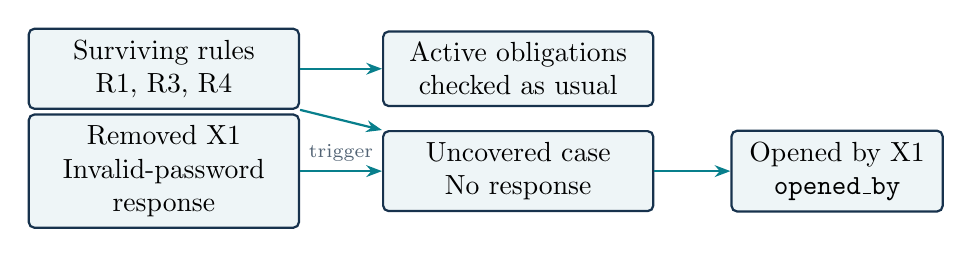
\begin{tikzpicture}[stage/.append style={font=\normalsize,text width=3.15cm,minimum height=8mm,inner sep=4pt}]
\node[stage] (active) at (0,0) {Surviving rules\\R1, R3, R4};
\node[stage] (check) at (4.5,0) {Active obligations\\checked as usual};
\node[stage] (removed) at (0,-1.3) {Removed X1\\Invalid-password response};
\node[stage] (seed) at (4.5,-1.3) {Uncovered case\\No response};
\node[stage,text width=2.4cm] (finding) at (8.55,-1.3) {Opened by X1\\\texttt{opened\_by}};
\draw[flow] (active)--(check);
\draw[flow] (active.south east)--(seed.north west);
\draw[flow] (removed)--node[above,font=\scriptsize,text=Muted]{trigger}(seed);
\draw[flow] (seed)--(finding);
\end{tikzpicture}

\par\endgroup
\vspace{-2mm}
\begin{columns}[T,onlytextwidth]
\column{.47\textwidth}
\begin{lstlisting}
Illustrative selected fields:
  "type": "gap",
  "opened_by": ["X1"],
  "about_change": true
\end{lstlisting}
\column{.49\textwidth}
Incorrect password submitted; account unlocked; failed-attempt count zero. No surviving conditional response applies.
\end{columns}
\takeaway{X1 supplies a former trigger to investigate; its obligation is no longer active.}\par\details{app-i}{I}\qquad\details{app-h}{H}
\talknote{1:15}{This is the same constructed authentication gap introduced in the early definitions. Start with R1--R4 only, remove the invalid-password response R2, and use X1 as an illustrative full-mode removal label. The actual full merger can renumber surviving R labels, so the diagram keeps the teaching labels rather than claiming a literal merged-label output. The remaining R1 and R4 still react to password submission. The old R2 antecedent p and not v points to the uncovered case; at p=true,v=false,locked=false,n=0, none of R1,R3,R4 applies. opened_by attributes that case to the deletion. This was checked offline against the archived implementation, not generated by a fresh LLM run. Removing the event's last conditional response is treated as retirement; state-only removals and replaced scenarios do not use the same removal-seeding mechanism.}
\end{frame}

\subsection{Reusing a saved base}

% MAIN 20 / 31

\begin{frame}[label=main20]{Reusing a saved base}
\begin{center}
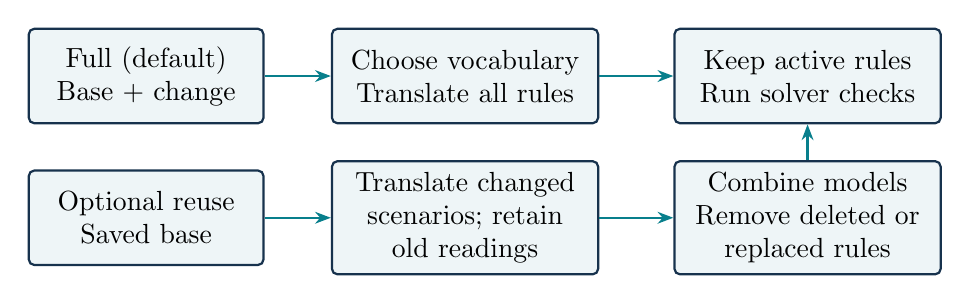
\begin{tikzpicture}[stage/.append style={font=\normalsize,minimum height=12mm,inner sep=4pt}]
\node[stage,text width=2.7cm] (full) at (0,0) {Full (default)\\Base + change};
\node[stage,text width=3.1cm] (translate) at (4.05,0) {Choose vocabulary\\Translate all rules};
\node[stage,text width=3.1cm] (check) at (8.4,0) {Keep active rules\\Run solver checks};
\node[stage,text width=2.7cm] (base) at (0,-1.8) {Optional reuse\\Saved base};
\node[stage,text width=3.1cm] (new) at (4.05,-1.8) {Translate changed\\scenarios; retain\\old readings};
\node[stage,text width=3.1cm] (combine) at (8.4,-1.8) {Combine models\\Remove deleted or\\replaced rules};
\draw[flow] (full)--(translate);\draw[flow] (translate)--(check);
\draw[flow] (base)--(new);\draw[flow] (new)--(combine);
\draw[flow] (combine)--(check);
\end{tikzpicture}

\end{center}
\vspace{-1mm}
\textbf{Authentication again:} keep the lockout readings; translate the exception.\par
Build the base once; rebuild when base text or model name changes.
\takeaway{Reuse keeps old interpretations while rerunning solver checks.}\par\vspace{0.25mm}\details{app-j}{J}
\slidesource{speccheck/cli.py: _base_model; speccheck/formalize.py: formalize; speccheck/probe.py}
\talknote{1:15}{Full formalization remains the default. Incremental mode first builds or loads a saved formal model of the labelled base specification, then translates only added or rewritten scenarios and probes the new rules. It combines those readings with the base, removes deleted and replaced obligations and their tagged assumptions, and reruns normal solver analysis. Cache reuse requires the same labelled base text and model-name string. Initial construction or invalidation costs a base formalization. This optimizes repeated alternatives against one base; after archiving a change into the base, the next check normally rebuilds it. Retaining interpretations is a semantic tradeoff, not incremental solver execution.}
\end{frame}

\section{Evaluation}

\subsection{Datasets and setup}

% MAIN 21 / 31

\begin{frame}[label=main21]{Datasets and setup}
\begin{tabularx}{\textwidth}{@{}lX@{}}
\toprule
Corpus & What is counted \\
\midrule
Ordinary specifications & 66 base documents; 297 versions; 11 sets \\
OpenSpec, separately & 18 projects; 102 distinct changes \\
Repeated runs & 3 per version or change \\
Main model & Qwen3.8-27B-FP8, served by vLLM \\
\bottomrule
\end{tabularx}
\takeaway{These project-authored test cases go beyond the small walkthrough examples.}
\par\vspace{0.25mm}\details{app-k}{K}
\slidesource{research.md: sections 1, 4.7; experiments/evaluate.py}
\talknote{1:00}{These project-authored datasets contain planted conflicts, gaps and ambiguities, with clean counterparts. There are 66 base documents, 297 versions and 11 sets in the ordinary-specification collection; OpenSpec separately has eighteen projects and 102 distinct changes across E17, E19 and E20. Each version or change is repeated three times. Thirty- and hundred-rule scale exercises and the three original examples are separate. Historical sets used different pipeline versions; they are not all experiments generated at revision 498dea0. E20 tests the same thirty-six changes in two modes; those are not seventy-two distinct changes. E19 froze its implementation before running eval13; E20 tested revision 373ae4c before the latest cache guards. The current offline suite has seventy passing tests. The four questions concern conflicts and extra alarms, ambiguities and extra questions, changes, and scale.}
\end{frame}

\subsection{Measures}

% MAIN 22 / 31

\begin{frame}[label=main22]{Measures}
\begin{tabularx}{\textwidth}{@{}lXl@{}}
\toprule
Measure & Criterion & Unit \\
\midrule
Conflict hit & Expected rule-position set is found & opportunities \\
Gap hit & Expected uncovered event is found & opportunities \\
Clean conflict alarm & A clean run has at least one alarm & runs \\
Ambiguity flag & Interpretation uncertainty is flagged & rules \\
\bottomrule
\end{tabularx}\par
\vspace{1mm}
Default counts include doubtful conflicts. Filtered counts are separate.
\takeaway{Unplanted flags need review before we call them false positives.}
\par\vspace{0.25mm}\details{app-k}{K}
\slidesource{experiments/evaluate.py; research.md: sections 1, 4.7}
\talknote{1:00}{Planted conflict hits match the expected set of rule positions. Gap scoring checks the event associated with the missing case. Clean conflict alarms count runs with at least one alarm, while ambiguity flags count rules across runs. E17's reported clean-change measure also includes covered-event gap alarms. Do not mix these denominators. Three repeated runs mainly expose translation variation, not three independent requirements problems. Clean ambiguity flags are unplanted and unadjudicated.}
\end{frame}

\subsection{Conflicts and extra alarms}

% MAIN 23 / 31

\begin{frame}[label=main23]{Conflicts and extra alarms}
\vspace{0pt}
{\small E18: six new domains. 12 planted conflicts $\times$ 3 runs; 6 clean specs $\times$ 3 runs.\par}
\begin{columns}[T,onlytextwidth]
\column{.49\textwidth}
\centering
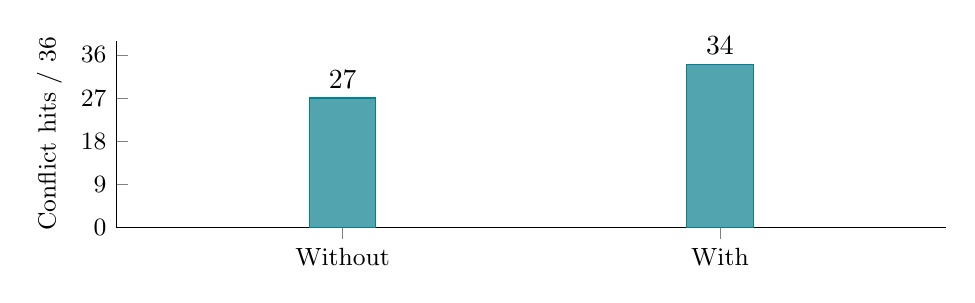
\begin{tikzpicture}
\begin{axis}[width=\linewidth,height=3.95cm,ybar,bar width=24pt,ymin=0,ymax=39,ytick={0,9,18,27,36},xmin=-.6,xmax=1.6,xtick={0,1},xticklabels={Without,With},ylabel={Conflict hits / 36},axis lines*=left,tick label style={font=\small},label style={font=\small},nodes near coords,every node near coord/.append style={font=\normalsize},enlarge x limits=false]
\addplot[fill=Teal!70,draw=Teal] coordinates {(0,27)(1,34)};
\end{axis}\end{tikzpicture}
\column{.49\textwidth}
\centering
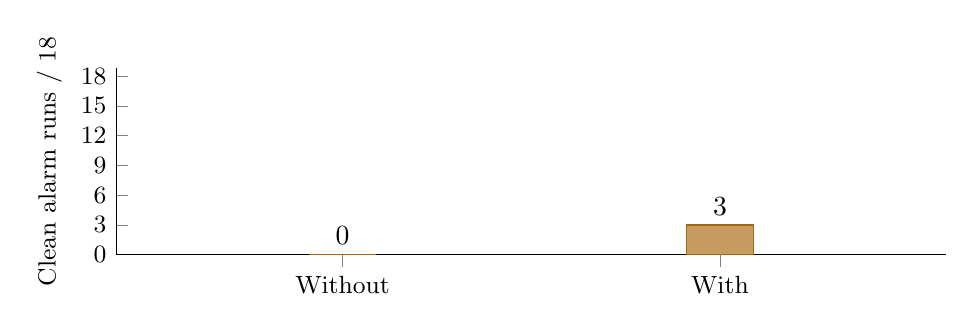
\begin{tikzpicture}
\begin{axis}[width=\linewidth,height=3.95cm,ybar,bar width=24pt,ymin=0,ymax=18.8,ytick={0,3,6,9,12,15,18},xmin=-.6,xmax=1.6,xtick={0,1},xticklabels={Without,With},ylabel={Clean alarm runs / 18},axis lines*=left,tick label style={font=\small},label style={font=\small},nodes near coords,every node near coord/.append style={font=\normalsize},enlarge x limits=false]
\addplot[fill=Amber!65,draw=Amber] coordinates {(0,0)(1,3)};
\end{axis}\end{tikzpicture}
\end{columns}
\vspace{-2mm}
Same saved runs, scored without/with outcome-pair facts.\\Bed conflict recovered. Extra alarm: collecting a previously unclaimed coat.\par\vspace{0.25mm}\details{app-e}{E}\qquad\details{app-k}{K}
\slidesource{experiments/results/E18_eval12.md; research_log.md: E18}
\talknote{1:30}{E18 was held out at the time and had 108 runs across six new domains. This is a scoring ablation on the same saved formalizations, not independently sampled pipelines. Default counts include doubtful conflicts. The change from 27/36 to 34/36 is seven more conflict/run detections, not seven distinct defects. Direct hits rose 9/18 to 16/18; overlap remained 18/18. Unexpected findings across all versions rose 1 to 28, or 0 to 27 after filtering doubtful findings. One temporal cloakroom pair explains 24 of the 27 added unexpected findings and all three clean-run alarms. Gaps were 17/18 and ambiguity hits 16/36 in both settings.}
\end{frame}

\subsection{Ambiguity and extra questions}

% MAIN 24 / 31

\begin{frame}[label=main24]{Ambiguity and extra questions}
\vspace{-1mm}
\begin{center}
\begin{tabular}{@{}lrr@{}}
\toprule
Measure & Main model & + second reader \\
\midrule
E9 planted ambiguities & 14/36 & 30/36 \\
E9 clean-rule flags (18 runs) & 7 & 15 \\
\addlinespace
E12 planted ambiguities & 17/36 & 32/36 \\
E12 clean-rule flags (18 runs) & 5 & 9 \\
\bottomrule
\end{tabular}
\end{center}
\vspace{-1mm}
``Open the gate and show the photo if the pass is a season pass.''\\Does \emph{if} govern the photo, or both actions?
\par{\small Reader: \code{thelamapi/next-70b}; unadjudicated flags; shortened example.\par}\par\vspace{0.25mm}\details{app-f}{F}
\slidesource{experiments/results/E9_eval4.md; experiments/results/E12_eval7.md}
\talknote{1:15}{The second model was thelamapi/next-70b in two separate 72-run experiments. Each clean-spec flag count is a count of rules across eighteen clean runs, not a percentage of runs. The flags are unplanted ambiguities and have not been independently adjudicated as false positives. The ski-pass sentence is an example of attachment ambiguity beyond numeric thresholds. Greater sensitivity also gives the reviewer more questions.}
\end{frame}

\subsection{Removal attribution}

% MAIN 25 / 31

\begin{frame}[label=main25]{Removal attribution}
\vspace{0pt}
{\small E19: 36 changes in six projects, repeated three times. Full formalization.\par}
\begingroup\centering\small
\begin{tabular}{@{}lr@{}}
\toprule
Measure & Result \\
\midrule
Planted conflicts found & 18/18 \\
Whole-requirement removal gaps & 18/18 \\
Dropped scenarios / narrowed coverage & 17/18 \\
Quiet changes with a conflict / gap alarm & 2/54\quad /\quad 0/54 \\
Runs with old conflict found and excluded & 108/108 \\
\bottomrule
\end{tabular}
\par\endgroup
{\small Excluding doubtful conflicts leaves 15/18. Quiet changes include retirements and edits to sibling scenarios.\par}
\takeaway{Removal attribution works on these cases; one lost condition hid a gap.}\par\vspace{0.25mm}\details{app-i}{I}\qquad\details{app-k}{K}
\slidesource{experiments/results/E19_eval13.md; research_log.md: E19}
\talknote{1:15}{E19 was frozen at 07ecd38 before eval13 was run. Whole-requirement removals produced 18/18 gap detections, while dropped scenarios or narrowed coverage produced 17/18. In the missed dorm case a retained rule lost a condition during translation and covered the gap. The two quiet conflict alarms concern a reworded makerspace sibling scenario; textual change tracking does not establish semantic novelty. Quiet changes total eighteen distinct cases repeated three times, including clean edits, event retirement and sibling edits. The old-conflict result is 108 run opportunities over six old conflicts, not 108 distinct defects. Earlier E17 evidence is retained in Appendix K.}
\end{frame}

\subsection{Reuse: requests and detections}

% MAIN 26 / 31

\begin{frame}[label=main26]{Reuse: requests and detections}
\vspace{0pt}
\setlength{\parskip}{2pt}
{\small E20: 36 new changes, each tested in both modes; three runs each.\par}
\begingroup\centering\small
\begin{tabular}{@{}lrr@{}}
\toprule
Measure & Full & Reuse \\
\midrule
Planted conflicts found & 54/54 & 50/54 \\
After doubtful conflicts are excluded & 51/54 & 45/54 \\
Planted gaps found & 36/36 & 36/36 \\
Clean changes with conflict / gap alarms & 0/18 & 0/18 \\
\addlinespace
Mean formalization requests per change & 68 & 9 \\
\bottomrule
\end{tabular}
\par\endgroup
\textbf{Initial base: about 61 extra requests on average.}\\
{\small Formalization only; excludes explanation and scenario judging.\par}
\takeaway{Reuse saves translation work, but missed four conflict detections here.}\par\vspace{0.25mm}\details{app-j}{J}\qquad\details{app-k}{K}
\slidesource{experiments/results/E20_eval14_full.md; experiments/results/E20_eval14_incremental.md; experiments/evaluate.py}
\talknote{1:30}{These are conflict-by-run detections, not independent defects. The four missed detections concern two cases: driving-school overlap in all three repetitions and a brewery direct conflict once. Reading the new driving-school rule alone could add an unstated registration-event condition, losing the clash or rejecting the reading. Both modes found all planted gaps. Zero alarms on the eighteen clean runs does not mean no extra findings elsewhere: total gap findings were thirty-nine versus forty-two and other change-related conflicts three versus one. Reuse used 1010 change requests plus 1093 base requests versus 7336 full-mode requests, about 71 percent fewer in this six-alternatives-per-base batch. Per-change means 68 and 9 are rounded; each initial base averaged 61 requests. The experiment tested 373ae4c; HEAD's model-name cache check and stricter option guards came afterward. No equivalence in semantic accuracy is established.}
\end{frame}

\subsection{Larger specifications}

% MAIN 27 / 31

\begin{frame}[label=main27]{Larger specifications}
\begin{tabularx}{\textwidth}{@{}lX@{}}
\toprule
30-rule campsite & Saved models: solver 26--34 s $\to$ 0.4--0.9 s by skipping unrelated rule families. \\
\addlinespace
100-rule ferry & Extracted count: 12/12 runs. Conflict hits 6/6; gaps 3/3; clean conflict alarms 1/3. \\
\addlinespace
Ferry, individual runs & Solver: 35 s. Full CLI: 620 s $\approx$ 10 min on a busy server. \\
\bottomrule
\end{tabularx}\par
\vspace{2mm}
Ferry failure: one symbol conflates a new reservation with an old seat release.
\takeaway{These timings and detection rates apply to the tested cases.}\par\vspace{0.25mm}\details{app-k}{K}
\slidesource{research_log.md: E13, E14}
\talknote{1:00}{Campsite has weakly connected subjects, so skipping unrelated rule combinations saves much work; a dense specification may benefit less. Ferry needed a larger extraction allowance after one answer reached 16,799 tokens. One of three clean ferry runs had a conflict alarm. The 35-second solver run and 620-second whole CLI run are individual observations, not latency averages. Second-reader context limits and the forty-pair cap matter at this size.}
\end{frame}

\section{Limitations and next steps}

\subsection{Representation limits}

% MAIN 28 / 31

\begin{frame}[label=main28]{Representation limits}
\lead{A coat can be listed as unclaimed, then collected later.}
\begin{center}

\begin{tikzpicture}
\node[slidetext] (a) at (0,0) {earlier\\unclaimed};
\node[slidetext] (b) at (5.2,0) {later\\released};
\draw[slidearrow] (a)--node[above,font=\normalsize]{time passes}(b);
\end{tikzpicture}
\end{center}
\vspace{3mm}
A single snapshot can make these outcomes look incompatible.\par
\vspace{1mm}
Payroll: setting \code{retention_years} to 10 does not say that deletion is forbidden.
\takeaway{More samples cannot recover a distinction that the vocabulary cannot express.}\par\vspace{0.25mm}\details{app-e}{E}
\slidesource{research_log.md: E18; research.md: sections 4.4--4.7}
\talknote{1:00}{The coat case is an observed E18 failure, not a hypothetical example. One snapshot loses the distinction between an earlier unclaimed state and later collection. The payroll example also shows that retention_years=10 is a value, not an obligation prohibiting deletion. Temporal and entity distinctions cannot be fixed by taking more samples of the same inadequate vocabulary. Temporal modeling is outside the baseline plan.}
\end{frame}

\subsection{Limits of reuse}

% MAIN 29 / 31

\begin{frame}[fragile,label=main29]{Limits of reuse}
\lead{Illustrative edit: change the sentence, keep the scenarios.}
\begin{lstlisting}
Before: The system SHALL retain records for five years.
After:  The system SHALL retain records for ten years.
Scenarios: unchanged
\end{lstlisting}
\textbf{Current incremental behaviour:} no new scenario text to translate; the saved base can be reused. Use full mode for this edit.
\vspace{0mm}
\begin{tabularx}{\textwidth}{@{}lX@{}}
\toprule
Search & Trigger groups stop at three; queries can return unknown. \\
Evidence & Independent specifications and reviewer studies are still needed. \\
\bottomrule
\end{tabularx}
\takeaway{No alarm does not establish that the requirements are correct.}\par\vspace{0.25mm}\details{app-j}{J}\qquad\details{app-k}{K}
\slidesource{speccheck/change.py: _document; speccheck/cli.py; offline sentence-only probe; constructed wording}
\talknote{1:15}{The wording is a constructed illustration of an offline-confirmed limitation. Incremental extraction emits only added or rewritten scenarios. A sentence-only requirement edit with unchanged scenarios emits no new text, and adding a requirement with no scenarios does likewise. Full mode includes those sentences. The CLI does not automatically fall back to full mode. If a base separately extracted an unlabelled SHALL obligation, scenario replacement tracking does not retire that old sentence-level obligation. Shared vocabulary and retained readings can also preserve an interpretation that is no longer suitable. Query timeouts, three-trigger groups and forty outcome-pair limits remain. An alternative reading can overlap only part of a gap; the annotation does not prove full coverage. Human time savings and explanation faithfulness have not been independently measured.}
\end{frame}

\subsection{Next work}

% MAIN 30 / 31

\begin{frame}[label=main30]{Next work}
\begin{tabularx}{\textwidth}{@{}rX@{}}
\textcolor{Teal}{\Large 1} & \textbf{Test beyond our own examples.}\\[-1mm]
 & Set aside fresh cases; add independent specs and reviewer decisions.\\[3mm]
\textcolor{Teal}{\Large 2} & \textbf{Make change checking practical.}\\[-1mm]
 & Handle sentence-only edits; test cache invalidation and detection loss.\\[3mm]
\textcolor{Teal}{\Large 3} & \textbf{Choose better symbols.}\\[-1mm]
 & Express retention obligations; flag lifecycle mix-ups; test the pair cap.\\
\end{tabularx}\par
\vspace{2mm}
Removal attribution and optional reuse are implemented.\\The next step is broader evidence and more complete edit handling.\par\vspace{0.25mm}\details{app-i}{I}\qquad\details{app-k}{K}
\slidesource{plan.md; docs/management/sections/next-steps.tex}
\talknote{1:00}{These priorities reflect revision 498dea0 without delivery dates or staffing commitments. Removal attribution and optional saved-model reuse have now been implemented and evaluated. First set aside fresh cases, since existing sets have become development data, and include independently adjudicated specifications. Then improve sentence-level edit handling and cache invalidation, and measure where reused interpretations lose detections. Finally improve the vocabulary for retention obligations and lifecycle distinctions and test the outcome-pair cap. The offline suite has seventy passing tests; those engineering checks do not validate natural-language interpretation.}
\end{frame}

\subsection{Conclusions}

% MAIN 31 / 31

\begin{frame}[label=main31]{Conclusions}
\begin{tabularx}{\textwidth}{@{}rX@{}}
\textcolor{Teal}{\Large 1} & \textbf{Solver findings can be traced back to requirements.}\\[-1mm]
 & Authentication connects text, formulas, a triggering case and saved evidence.\\[4mm]
\textcolor{Teal}{\Large 2} & \textbf{Interpretation and reuse choices have measurable tradeoffs.}\\[-1mm]
 & E18 improves detection with extra alarms; E20 saves requests but misses conflicts.\\[4mm]
\textcolor{Teal}{\Large 3} & \textbf{The current evidence supports further evaluation.}\\[-1mm]
 & Independent specifications and reviewer studies are the next test.\\
\end{tabularx}\par
\vspace{1mm}
The scope remains requirements review under an explicit snapshot model.
\par\vspace{0.25mm}\details{app-a}{A}
\slidesource{research.md; research_log.md; speccheck/checks.py; speccheck/explain.py}
\talknote{0:45}{The three conclusions follow the research question. First, the pipeline retains concrete evidence linking requirements to logical findings. Second, extra interpretation checks recovered more planted cases and also raised more questions and alarms. Removal attribution now follows deleted rules into gap findings. E20 additionally shows a request-saving reuse mode with lower conflict detection than the full run. Third, the project-authored experiments justify further evaluation, not claims of production quality or measured human benefit. The appendix contains the complete model, procedures, reuse constraints and replay limits.}
\end{frame}

% TECHNICAL APPENDIX: 11 frames, outside the main talk.

\appendix

\mainframefalse

\section*{Technical appendix}

\begin{frame}[noframenumbering,label=app-a]{A. The authentication model}
\backuptext
\begin{columns}[T,onlytextwidth]
\column{.46\textwidth}
\begin{tabular}{@{}cl@{}}
\toprule
$p$ & password submitted \\
$v$ & password correct \\
$g$ & access granted \\
$d$ & access denied \\
$n$ & failed-attempt count \\
$\ell$ & account locked \\
$h$ & administrator account \\
\bottomrule
\end{tabular}
\column{.50\textwidth}
\textbf{Baseline, selected readings}\par
\begin{align*}
\phi_1&=(p\land v)\Rightarrow g\\
\phi_2&=(p\land\neg v)\Rightarrow d\\
\phi_3&=(n=5)\Rightarrow\ell\\
\phi_4&=(p\land\ell)\Rightarrow d
\end{align*}
\textbf{Proposed addition}\quad $\phi_5=h\Rightarrow\neg\ell$
\end{columns}
{\small R3's alternative is $(n\ge5)\Rightarrow\ell$. Grant and deny are separate symbols.\par}
One valuation is one snapshot. The constructed gap removes R2 from the baseline.\par\backto{main05}{the predicates}
\note{These abbreviations match selected formulas in specs/auth_change/formal.json at the preserved revision. The baseline illustration projects R1--R4 from that saved combined model; it is not an independently sampled base run. The full order model is retained in the paper as a separate worked example. R3's actual antecedent is n=5 without p. The selected R3 reading and its alternative are not asserted equivalent.}
\end{frame}

\begin{frame}[noframenumbering,label=app-b]{B. Extraction, sampling and grouping}
\backuptext
\begin{algorithmic}[1]
\State Ask for atomic rules, copied text, IDs, triggers and typed symbols
\State Retry reading at temperatures $0,0.3,0.9$; fail without usable vocabulary
\ForAll{rules, with up to sixteen concurrent requests}
 \State Request $N=8$ translations using the same vocabulary; temperature $0.7$
\EndFor
\State Parse formulas serially; discard malformed translations; reject if none remain
\ForAll{usable translations $\psi$}
 \State Join a cluster represented by $\phi$ only if $\UNSAT(\phi\oplus\psi)$
 \State Otherwise start a new cluster
\EndFor
\State For cluster sizes $m_j$, set $p_j=m_j/\sum_\ell m_\ell$ and $H=-\sum_jp_j\ln p_j$
\State Accept if $H\le0.4$; ambiguous if $0.4<H\le1$; otherwise reject
\State Select the shortest formula in the largest cluster; retain an alternative if needed
\end{algorithmic}
\vspace{0mm}
Illustration: $[5,3]$ gives $H\approx0.662$. Eight identical mistakes would give $H=0$.\par\vspace{0.25mm}\backto{main12}{sampling and grouping}
\slidesource{speccheck/formalize.py: _read, _translate, _judge, _group_by_meaning}
\note{Entropy divides by usable translations, unlike the requested-sample denominator for fact and link majority votes. A rule with no usable cluster is rejected. Only solver-proved equivalence merges translations; unknown does not. The shortest expression is chosen from the largest cluster. When not accepted, retain the next cluster if available and seek a distinguishing witness. Types and JSON validity do not establish that the vocabulary captures the intended concepts.}
\end{frame}

\begin{frame}[noframenumbering,label=app-c]{C. Assumed facts and outcome links}
\backuptext
\begin{columns}[T,onlytextwidth]
\column{.48\textwidth}
\textbf{Facts from symbol descriptions}
\begin{algorithmic}[1]
\State Ask $N$ answers; parse and discard answer sets proved inconsistent
\State Count support by logical entailment, not matching text
\State Retain candidates supported by $>N/2$ answers
\State Skip tautologies, implied facts and facts proved inconsistent with retained assumptions
\end{algorithmic}
\column{.48\textwidth}
\textbf{Links from restating a rule}
\begin{algorithmic}[1]
\State Hide a private outcome; request $N$ restatements in other symbols
\State Group usable answers by equivalence
\State Require a cluster with $>N/2$ answers
\State From $a'_i\Rightarrow c'_i$, propose $(a'_i\land c_i)\Rightarrow c'_i$
\State Retain unless proved inconsistent with assumptions
\end{algorithmic}
\end{columns}
\vspace{1mm}
D2: $d\Rightarrow m$; restate as $d\Rightarrow\neg k$; link: $(d\land m)\Rightarrow\neg k$.
\takeaway{Both mechanisms add assumptions that later probes can challenge.}\par\vspace{0.25mm}\backto{main13}{outcome assumptions}
\slidesource{speccheck/formalize.py: _agreed_facts, _symbols_to_hide, _links}
\note{Both majority thresholds use requested N; missing answers count against support. Facts are ranked by support and then formula length. A link is retained even if existing facts imply it, since those facts may later be rejected. Unknown is not proof of inconsistency or entailment. During incremental reuse, facts are asked again only when new symbols appear, and restatements cover only new rules.}
\end{frame}

\begin{frame}[noframenumbering,label=app-d]{D. Probing readings, links and facts}
\backuptext
\begin{algorithmic}[1]
\State Propose at most three alternatives for each accepted rule
\State For an ambiguous rule, use the alternative from its sampled clusters
\State Remove equivalent/invalid alternatives; proposed ones use existing rule symbols
\State Seek $\phi\land\neg\psi$ and $\neg\phi\land\psi$ witnesses
\State Ask eight answers across witnesses and reversed A/B presentation orders
\State Chosen reading stands if it wins $>1/2$ of usable replies, or none return
\State Confirm a link if most replies forbid its violating witness, or none return
\State Reject a suspect fact only if most replies say it contradicts the rule
\end{algorithmic}
\vspace{2mm}
$n=6$, $\ell=\False$ separates the two readings. If the alternative wins, flag an ambiguity; keep the original rule.\par\vspace{0.25mm}\backto{main08}{checking readings}
\slidesource{speccheck/probe.py: question, _other_readings; speccheck/checks.py: settled}
\note{Witnesses are first sought under domain facts, then without them if necessary. If the chosen reading stands against every tested alternative it becomes accepted; otherwise ambiguous. Rejected translations remain rejected. No replies is the implementation's explicit preserve/accept fallback, not positive evidence.}
\end{frame}

\begin{frame}[noframenumbering,label=app-e]{E. Outcome-pair questions}
\backuptext
\begin{algorithmic}[1]
\ForAll{pairs of usable rules in document order}
 \State Skip antecedents proved incompatible under retained assumptions
 \State Skip pairs reacting to disjoint events
 \State Require disjoint outcome symbols and definite outcome assignments
 \State Skip outcomes proved incompatible under assumptions
\EndFor
\State Ask about the first forty eligible pairs, eight answers per pair
\ForAll{selected pairs $(i,j)$}
 \If{more than half of its usable answers say ``impossible''}
  \State Add assumed fact $\neg(c_i\land c_j)$ and record rule IDs/support
 \EndIf
\EndFor
\end{algorithmic}
\vspace{2mm}
Constructed bed vote: 6 impossible, 2 possible. Keep the assumed exclusion.\par
Conditional retention or a numeric bound may not be definite.\par\vspace{0.25mm}\backto{main23}{conflict evaluation}
\slidesource{speccheck/probe.py: outcomes, _open_pairs, _as_facts}
\note{The illustrative bed vote has six impossible and two possible answers. E18 asked 410 eligible pairs and 58 got majority-impossible replies. The cap is important for large documents. This mechanism recovered release/hold and cloakroom retention conflicts, but also introduced the temporal unclaimed/collected artefact.}
\end{frame}

\begin{frame}[noframenumbering,label=app-f]{F. Check readings and vocabulary}
\backuptext
\textbf{Second reader, same vocabulary}
\begin{algorithmic}[1]
\State Translate each usable rule $N$ times with another model
\State Find event symbols $E_i$ entailed by the original antecedent
\State Count $\psi_j$ with $\UNSAT(\bigwedge E_i\land(\phi_i\oplus\psi_j))$
\State Confirm if count $>N/2$; otherwise retain a usable other reading
\State New ambiguity needs both failed confirmation and an alternative
\end{algorithmic}
\vspace{3mm}
\textbf{Repeated vocabulary selection}
\quad Match conflicts by rule set and ambiguities by rule ID. A finding in $k$ of $K$ retained models has support $k/K$; retain gaps from the first model.
{\small Illustrative second reader: $3/8$ exactly five, $5/8$ five or more.\par}
\takeaway{These options require full mode; incremental mode excludes them.}\par\vspace{0.25mm}\backto{main24}{ambiguity evaluation}
\slidesource{speccheck/formalize.py: formalize_sets, judge_second; speccheck/checks.py: combine}
\note{Additional vocabularies are currently aligned by rule count and position, not by verified text correspondence. A second model can disagree on exactly-five versus at-least-five while remaining limited by the original symbol inventory. Missing second-model answers count against requested N but alone provide no alternative to report. Agreement is not a probability of correctness. HEAD rejects incremental mode with multiple vocabularies, a second reader, or text review; it does not switch modes automatically.}
\end{frame}

\begin{frame}[noframenumbering,label=app-g]{G. Conflict search and explanations}
\backuptext
{\small $A_G=\bigwedge_{i\in G}a_i$: the selected triggering conditions.\par}
\begin{algorithmic}[1]
\For{$B=\varnothing$, then retained assumptions}
 \ForAll{trigger groups $G$, $1\le |G|\le3$, within connected symbol families}
  \State Skip supersets of previously conflicting triggers
  \State Require $\SAT(A_G\land\bigwedge B)$
  \State Continue unless all obligations with $A_G$ are proved unsatisfiable
  \State Extract an unsatisfiable core of rules and facts
  \State Try deleting each core member while preserving unsatisfiability
  \State Exclude cases where one rule alone forbids the trigger with $B$
  \State Record rule IDs, necessary assumptions and a trigger witness
 \EndFor
\EndFor
\State Deduplicate; assumptions may add findings or flag doubt, but cannot erase rules-only findings
\end{algorithmic}
\vspace{0mm}
R3 and R5 force $\ell\land\neg\ell$ when $A_G=h\land(n=5)$.\hfill\backto{main06}{conflicts}
\slidesource{speccheck/checks.py: _search, _families, _minimal_conflict}
\note{The core is deletion-minimized, hence subset-minimal with conclusive solver answers, not necessarily minimum cardinality. Five-second query timeouts can yield unknown, which is never asserted as a proof. No proof certificate is saved. The trigger-group bound is not a bound on core size.}
\end{frame}

\begin{frame}[noframenumbering,label=app-h]{H. Gaps and removed responses}
\backuptext
Surviving conditional rules $C$; handled event $e$. Ordinary search:
\par\vspace{1mm}
\hfill$\SAT\!\left(e\land\bigwedge_{e'\ne e}\neg e'\land\bigwedge_{i\in C}\neg a_i\right).$\hfill\mbox{}\par
\begin{algorithmic}[1]
\State Seed a case with a usable removed rule's antecedent/event context
\State Require an event still handled by a surviving conditional rule
\State Seek a case where no surviving antecedent holds; record \texttt{opened\_by}
\State Per event: removal-seeded gap if found, else ordinary gap; add one quiet gap
\State Prefer witnesses allowed by assumptions; otherwise mark doubt
\State Generalize only while every completion remains uncovered
\end{algorithmic}
\vspace{0mm}
At most one removal-seeded gap per event. Excludes state-only removals and retirement of an event's last response.
\takeaway{An alternative reading can leave part of a gap uncovered.}\par\vspace{0.25mm}\backto{main19}{the removal example}
\slidesource{speccheck/checks.py: find_gaps, find_scenarios, _try_other_readings}
\note{Rejected removed translations are skipped. Replaced scenarios are removed from active checks but are not seeds for this mechanism. No conditional rules means no gaps. Ordinary event search emits at most one gap per handled event and one quiet gap; without events the fallback seeks at most three generalized gaps. Unconditional rules constrain outcomes rather than supply coverage. For a sensitivity example, original (s and x) implies f has gap s=true,x=false, while alternative (s and y) implies f covers only y=true completions. The overlap test may also pass on solver unknown. Allowed scenarios instead satisfy all rule implications and an outcome outside its condition; an LLM ranks relevance and selects at most three.}
\end{frame}

\begin{frame}[noframenumbering,label=app-i]{I. Change checking}
\backuptext
\begin{algorithmic}[1]
\State Load base specs and delta; apply rename, remove, modify and add operations
\State Match scenarios by name and normalized text; retain textual provenance
\State Full mode: formalize the labelled combined document, including removed X rules
\State Reuse mode: combine the saved base and formalized new N scenarios
\State Validate that expected scenario labels appear exactly once
\State Separate removed/replaced obligations; prune links and pair facts referring to them
\State Analyze the active model, with true deletions available as gap seeds
\State Select conflicts/scenarios/ambiguities involving changed rules
\State Select gaps involving changed events or carrying \texttt{opened\_by}
\State Retain other findings in JSON without presenting them as the change's
\end{algorithmic}
\vspace{1mm}
Scenario matching is textual. Rewording a rule can still count as a change when its meaning is unchanged.\par\vspace{0.25mm}\backto{main17}{change analysis}
\slidesource{speccheck/change.py: merge, changed_rules, after_model, about_change; speccheck/cli.py}
\note{Unchanged scenario bodies retain existing provenance inside a modified requirement; comparisons ignore case, whitespace and selected Markdown differences. R labels identify surviving/full-mode scenarios; X labels identify removed full-mode scenarios; incremental new scenarios use N labels. Deleted requirements retain their SHALL text for matching unlabelled extracted rules. Replaced old scenarios are removed from active checks but are not removal-gap seeds. Ordinary voted domain facts remain; only assumptions tagged as restating or relating removed/replaced rules are pruned. Thus removed text can still influence full-mode extraction and ordinary domain facts. Neither changed-event relevance nor textual provenance is a general semantic causality proof.}
\end{frame}

\begin{frame}[noframenumbering,label=app-j]{J. Saved-base reuse}
\backuptext
\begin{algorithmic}[1]
\State Reject multiple vocabularies, a second reader, or text review with reuse
\State Compute a fingerprint of the labelled base document and the model name
\State Load the saved base if both match; otherwise formalize and save the base
\State Emit only added/rewritten scenarios as new text
\If{new text exists}
 \State Extend vocabulary; retain old definitions/readings; translate the new rules
 \State Probe new rules and eligible outcome pairs containing a new rule
 \State Combine with the saved base
\EndIf
\State Validate labels; remove deleted/replaced rules; run ordinary solver checks
\end{algorithmic}
\vspace{1mm}
Cache key: base text + model name. It omits sampling settings, endpoint and prompt/code changes. Invalid models abort without a full-mode fallback.
\takeaway{Use full mode for sentence-only edits or to reconsider old interpretations.}\par\vspace{0.25mm}\backto{main20}{the two execution modes}
\slidesource{speccheck/cli.py: _base_model; speccheck/formalize.py; speccheck/probe.py; speccheck/change.py}
\note{The key includes the SHA-256 of the generated labelled base document and the model-name string. The saved cache is openspec/.speccheck/base.json. First use or a mismatch rebuilds a base model, not a freshly formalized combined change. A supplied formal JSON bypasses this cache-validation branch. Old symbol definitions win over redeclarations. Facts are requested again only if new symbols appear; old rules are not all re-probed under new facts. Outcome-pair probing remains capped at forty eligible pairs. Sentence-only changes and new requirements without scenarios produce no incremental text. Empty new text still leads to projection and solver checking; the full CLI may call the LLM for explanations and scenario judging. E20 precedes HEAD's model-name guard and stricter option checks.}
\end{frame}

\begin{frame}[noframenumbering,label=app-k]{K. Historical evidence and replay}
\backuptext
\begin{tabularx}{\textwidth}{@{}lX@{}}
\toprule
E17, earlier change study & 36/36 conflicts; 33/36 excluding doubtful; 36/36 gaps; 0/18 clean alarms. Removal attribution was still limited. \\
E19 / E20 freezes & E19: \texttt{07ecd38}. E20: \texttt{373ae4c}. Later cache guards belong to the documented revision \texttt{498dea0}. \\
\bottomrule
\end{tabularx}\par
\vspace{1mm}
\textbf{Saved inputs:} \texttt{merged.md} records the combined change document; \texttt{new.md} records incremental scenario text; \texttt{base.json} holds the cached base.
\par
\textbf{Replay:} \texttt{formal.json} is saved before deleted/replaced rules are separated. Replay change preprocessing before running the active-model solver checks.
\takeaway{The snapshot preserves code and results, not model weights. Fresh model runs may differ.}\par\vspace{0.25mm}\backto{main22}{evaluation measures}
\slidesource{speccheck/cli.py; research_log.md; experiments/results/E17_eval11.md; docs/management/UPDATE.md}
\note{E17 tested thirty changes in six projects, repeated three times. Its clean measure includes conflict and covered-event gap alarms. The cinema case was doubtful because two modeled events had to coincide. Most older experiments lack the exact producing commit; do not assign them retroactively to HEAD. A raw formal model is not necessarily the post-change active model. Saved formulas support solver replay without a model server, but generating prose and judging scenarios require model calls. Reused formal JSON is not copied into replay output automatically. The snapshot records inputs explicitly. E20 counters measure formalization requests only; an initial base costs about sixty-one requests and archiving a change normally invalidates it.}
\end{frame}

\end{document}
